\section{AppCoins: Protocol Definition}
\label{sec:protocol}

As we have seen before, the AppCoins protocol addresses the use cases of Advertising, In-App Billing (IAB) and Developer Reputation within app stores by leveraging the blockchain construction to create value for the different participants.\\

In this section, we present the data structures and algorithms used to solve each of the aforementioned use cases. It will be organised as follows: a section for each core flow and subsections explaining the data structures, algorithms and wallets flows.

\subsection{Advertising}

Advertising campaigns in the context of a blockchain must be constructed in a way as to overcome the risks elaborated before.

\subsubsection{Use Case Flows}

Figure \ref{fig:ads_sequence_diagram} shows the interactions between the several parties that coexist in the Advertising use case.

\begin{figure}[H]
\centering
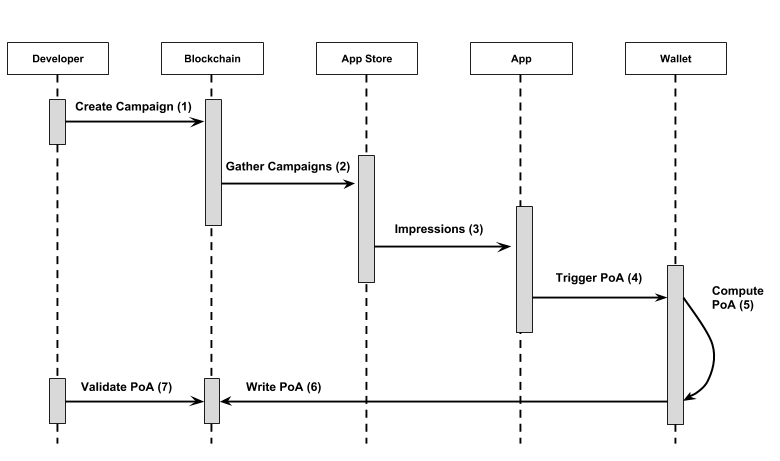
\includegraphics[width=\textwidth]{diagrams/ads_sequence_diagram.png}
\caption{Sequence diagram of the Advertising use case.}
\label{fig:ads_sequence_diagram}
\end{figure}


\noindent \textbf{Create Campaign (1)}. When developers (advertisers) want to create a campaign, they do so by creating an entry in the blockchain with all the required data to identify that campaign and the users that will be eligible to convert it. This data will contain information about the advertised package, the countries targeted by the campaign, the budget allocated by the developer to the campaign, the amount of \textsf{APPC} to be paid by attribution, the start and end dates of the campaign, and the IP validator of the users IPs. In addition, a campaign also contains information about the rules to be used in order to validate attributions to users. Also, when a campaign is created, the budget allocated to the campaign is transferred. That value is decreased by the amount of \textsf{APPC} sent to successful attributions. The campaign will remain active until there is no budget or the {\em end\_date} is reached. The way for a developer to cancel a campaign is to withdraw the existent funds. \\

\noindent \textbf{Gather Campaign (2) \& Install (3)}. When campaigns are saved in the blockchain, they will then be gathered by the app stores that match the filters of the campaign with their users. Upon matching, app stores then present the available campaigns to each user. It is important to mention that an app store should only show a campaign to a given user if and only if the user matches the campaign filters. If a user provides a \textsf{PoA} to a campaign with filters not matching the user's profile, the user will spend \textsf{APPC} to provide the \textsf{PoA} but will not be entitled to the attribution and the correspondent \textsf{APPC} because the provided \textsf{PoA} will be considered invalid by the protocol. In this case, the app store will see its earnings from the Advertising revenue share model lowered because users will realise the app store shows campaigns to users only with the intent of maximum profit. Users will then be compelled to move to other app stores to avoid the risk of losing the required amount of \textsf{APPC} when registering the campaigns \textsf{PoAs}.\\

\noindent \textbf{Trigger \textsf{PoA} (4)}. After the installation of an app by a user with a campaign associated with it, the SDK integrated in the app will trigger an AppCoins compliant wallet to compute the components of the \textsf{PoA}. It will trigger the wallet every 10 seconds during the 2 minutes needed to compute a valid \textsf{PoA}. For each trigger and for each consequent \textsf{PoA} component sent by the SDK, the wallet computes a \textit{nonce} in a Bitcoin-style proof-of-work (PoW) that serves to validate the component and help avoiding click spoofing. This process is detailed in Section \ref{sssec:ads_fd}. \\

\noindent \textbf{Compute \textsf{PoA} (5) \& Write \textsf{PoA} (6)}. After there are 12 components of a \textsf{PoA} for the same campaign computed within 2 minutes, the complete \textsf{PoA} is computed and written in the blockchain for registration and further validation. \\

\noindent \textbf{Validate \textsf{PoA} (7)}. The validation / invalidation of the \textsf{PoAs} is an optional part of the protocol where it is defined that a \textsf{PoA} is valid. If there is not an invalidation within 60 (sixty) minutes by the developer responsible by the creation of the campaign, the \textsf{PoA} is considered valid and the user is paid by the smart contract. Although it may carry a cost of the transaction fee, a quick validation by the developer would create a better user experience for the user, sine the reward would be attributed sooner.


\subsubsection{Data Structures}
\label{sssec:ads_ds}

\noindent \textbf{Campaign}. A \textit{Campaign} is a statement of intent to pay for the attention of users. Developers create \textit{campaigns} and submit them to the blockchain. App stores fetch open campaigns from the blockchain and propagate them to users. Campaigns are composed of an amount of funds, a duration, the amount of tokens per attribution and the filters (app name, app version, geolocation,...). Please refer to Table \ref{table: data_structures_ad} for more details. \\

\noindent \textbf{Advertising Ledger}. The \textit{advertising ledger} is the record of attributions, i.e. users that completed the required action (e.g. having an app open for at least 2 minutes) for a campaign. The ledger is populated in a way that avoids the \textit{double attribution problem}, i.e. attributions that come from different app stores for the same campaigns / apps in similar time intervals need to be identifiable across all the stores, as well as the users.

\begin{table}[H]
\footnotesize
\centering
\begin{tabular}{|p{.5\textwidth}p{.5\textwidth}|}
\hline
\multicolumn{2}{|c|}{Data Structures} \\
\hline \vspace{0.05cm}
\textbf{Campaign} & \vspace{0.05cm} \textbf{Advertising Ledger} \\
campaign $C_a : \langle F_{a}, \Delta t_{a}, T_{a}, filters, D_i \rangle$
\begin{itemize}
	\item Funds $F_{a}$, the amount of tokens the developer $D_{i}$ is willing to spend for $C_{a}$
	\item Duration $\Delta t_{a}$, the duration of $C_{a}$
	\item Tokens per attribution $T_{a}$, the amount of tokens to be sent from $D_{i}$ and distributed to the other parties per attribution
	\item Filters, the specifics of $C_{a}$, as the app name, app version, geolocation of $C_{a}$ and others available to $D_{i}$
	\item Developer $D_i$, developer that submitted a campaign $C_a$
\end{itemize} &
advertising ledger $L_{Ad} : (A^{1}_{t}..A^{n}_{t})$
\begin{itemize}
	\item Attribution $A^{i}_{t}$, $i$-th attribution in the advertising ledger $L$, which is composed as a mapping $A^{i}_{t} : \{C_{N}^{j} \to (U_{N}^{1}..U{N}^{n})\}$, where $C_{N}^{j}$ is the standardised campaign $C_a$ across all the app stores and $U_{N}^{i}$ is the normalised user $U_i$ across all the app stores
\end{itemize} \\
\hline
\end{tabular}
\caption{Data Structures for Advertising Use Case}
\label{table: data_structures_ad}
\end{table}


\subsubsection{Algorithms' Pseudo-code}

Table \ref{table: ads_use_case} presents in pseudo-code a more in-depth definition of the following methods. \\

\noindent \textbf{Create campaign}. When a campaign is submitted to the blockchain, the \textsf{CreateCampaign} method creates the campaign $C$ containing the all the parameters describing the campaign as the funds $F$, duration $\Delta t$, etc. In addition, the funds $F$ the developer wishes to allocate to the campaign are sent from the developer's wallet $W_D$ to the campaign's contract wallet $W_C$. Since the created campaign is in the blockchain accessible to every user, it is used to overcome the \textit{bid refutation} problem.\\

$\left[\begin{tabular}{p{.7\textwidth}}
\textsf{AD.CreateCampaign}
\begin{itemize}
	\item INPUTS:
	\begin{itemize}
		\item Campaign parameters:
		\begin{itemize}
			\item Funds $F$
			\item Duration $\Delta t$
			\item Tokens paid per attribution $T$
			\item Filters (geolocation, app name, app version,...)
		\end{itemize}
		\item Developer $D$
	\end{itemize}
	\item OUTPUTS: Campaign $C$
\end{itemize}
\vspace{-0.8cm}
\end{tabular}\right.$ \\

\noindent \textsf{Set attribution}. When a user has been attributed to a campaign $C$, i.e. the user performed the required action (e.g. had the app open for at least 2 minutes), \textsf{SetAttribution} checks the advertising ledger $L_{Ad}$ to make sure the user $u$ has not yet been attributed to the campaign $C$ and if so, the attribution is written in the ledger and each participant receives the correspondent tokens, i.e. the user, OEM and app store receive $T_u$, $T_{OEM}$ and $T_{AS}$, respectively. Since the method is constructed in a way such that the same user is unable to be attributed the same campaign in different app stores, it avoids the \textit{double attribution problem}. \\

$\left[\begin{tabular}{p{.5\textwidth}}
\textbf{AD.SetAttribution}
\begin{itemize}
	\item INPUTS:
	\begin{itemize}
		\item User $u$
		\item Campaign $C$
	\end{itemize}
	\item OUTPUTS: Result $R$ (0 or 1)
\end{itemize}
\vspace{-0.8cm}
\end{tabular}\right.$ \\

\begin{table}[H]
\scriptsize
\centering
\begin{tabular}{|p{.5\textwidth}p{.5\textwidth}|}
\hline
\multicolumn{2}{|c|}{Advertising Use Case} \\
\hline \vspace{0.1cm}
\textsf{AD.CreateCampaign}
\begin{itemize}
	\vspace{-0.3cm}
	\item INPUTS:
	\vspace{-0.4cm}
	\begin{itemize}
		\item Campaign parameters:
		\begin{itemize}
			\item Funds $F$
			\item Duration $\Delta t$
			\item Tokens paid per attribution $T$
			\item Filters (geolocation, app name,...)
		\end{itemize}
		\item Developer $D$
	\end{itemize}
	\item OUTPUTS: Campaign $C$
\end{itemize}
\begin{enumerate}
	\item Compute $C$ := \textsf{CreateCampaign}($F$, $D$, $\Delta t$, $T$, $filters$)
	\item Send $F$ from developer's wallet $W_D$ to campaign's wallet $W_C$
\end{enumerate} & \vspace{0.1cm} \textsf{AD.SetAttribution}
\begin{itemize}
	\vspace{-0.3cm}
	\item INPUTS:
	\vspace{-0.4cm}
	\begin{itemize}
		\item User $u$
		\item Campaign $C$
	\end{itemize}
	\item OUTPUTS: Result $R$
\end{itemize}
\begin{enumerate}
	\item Compute $InLedger$ := \textsf{CheckAdvertisingLedger}($u$, $C$)
	\item If $InLedger$ = 1:
	\begin{itemize}
		\item Set $R$ := 0
	\end{itemize}
	\item If $InLedger$ = 0:
	\begin{enumerate}
		\item Compute $TX$ := \textsf{Transaction}($u$, $C$)
		\item Compute $R$ := \textsf{WriteAdvertisingLedger}($TX$)
		\item Compute $(T_u, T_{OEM}, T_{AS})$ := \textsf{DivideTokens}($T$)
		\item Send $T_u$ to user's wallet $W_U$
		\item Send $T_{OEM}$ to OEM's wallet $W_{OEM}$
		\item Send $T_{AS}$ to user's wallet $W_{AS}$
	\end{enumerate}
\end{enumerate} \\
\hline
\end{tabular}
\caption{Advertising Use Case}
\label{table: ads_use_case}
\end{table}


\subsubsection{Wallet Transactions}

The transfers between wallets in the Advertising flow have to address some risks that were previously described in Chapter \ref{subsec:intro_ads}.

There is a wallet that contains the budget of the created campaign, which is meant to lock the budget, addressing the risk of default (R1.5) by the developer. To address the same risk, there is also a wallet that will temporarily store the value of the impression, to make sure that if the attribution occurs within a certain time, i.e. the user installs and opens the app within a certain time interval, there are funds available to pay for the conversion. Otherwise, there could be a scenario of serving an impression to many users but the campaign only had enough funds for one more attribution. The users would try to get attribution, creating a race condition, but only one would get it. An example of this schema is shown in Figure \ref{fig:wallet_cpi_flow}.

\begin{figure}[H]
\centering
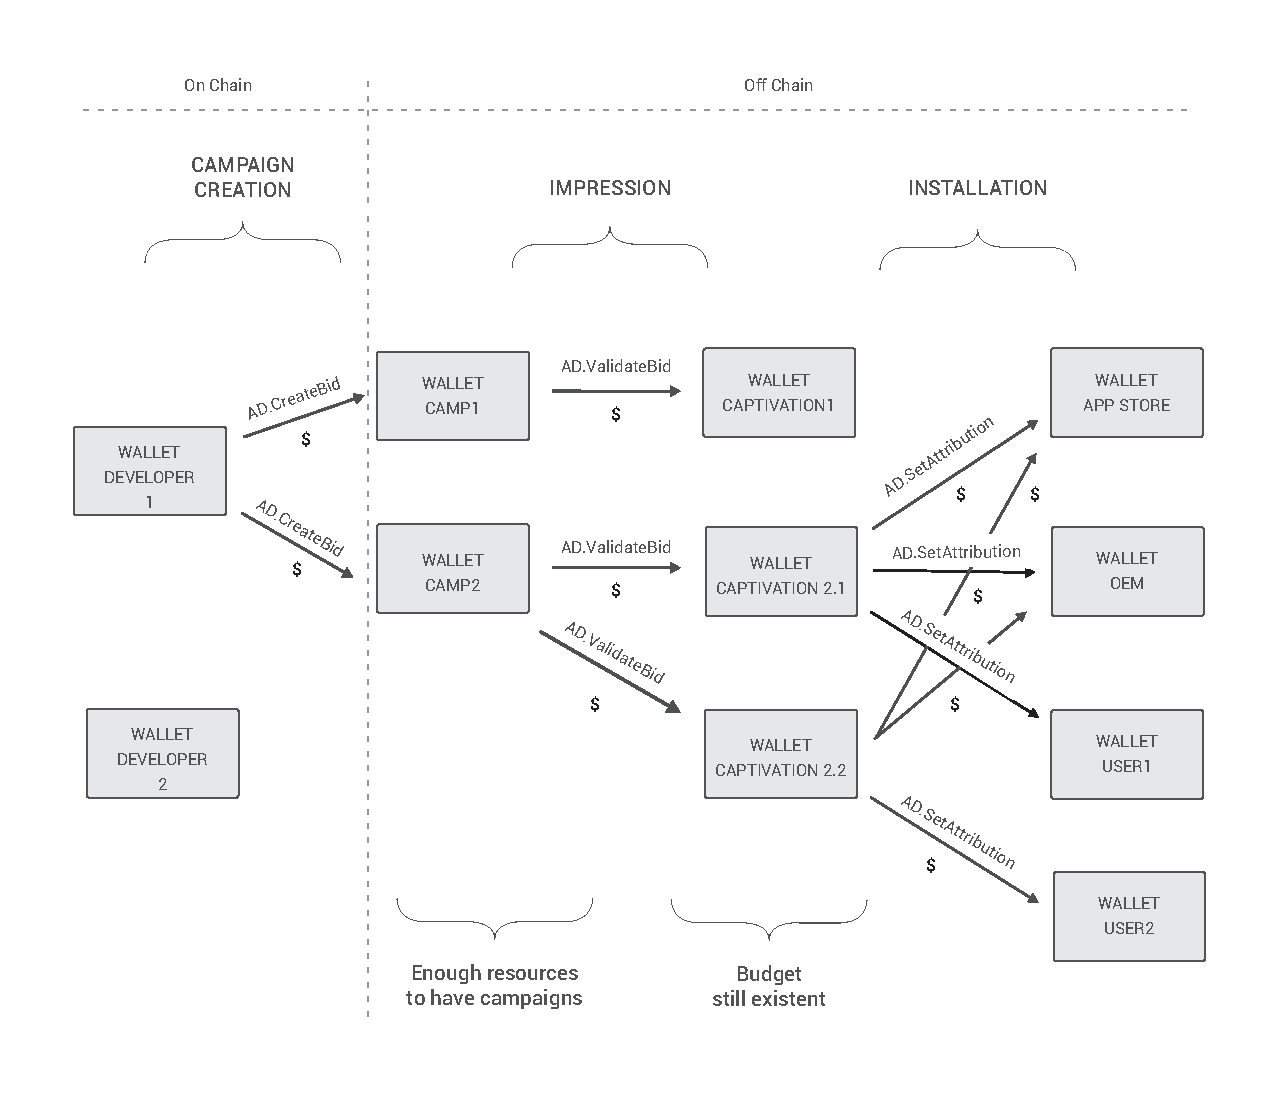
\includegraphics[width=\textwidth]{diagrams/wallet_transfers.eps}
\caption{Wallet transfers in the CPI advertising flow.}
\label{fig:wallet_cpi_flow}
\end{figure}

\subsubsection{Messages Format Definition}
\label{sssec:ads_fd}

This section details the format of the objects needed for the Advertising use case. To implement the protocol one needs to be compliant with these messages to assure interoperability of the different components. \\

The messages and data structures exchanged are:

% insert diagram with structures
\begin{figure}[H]
\centering
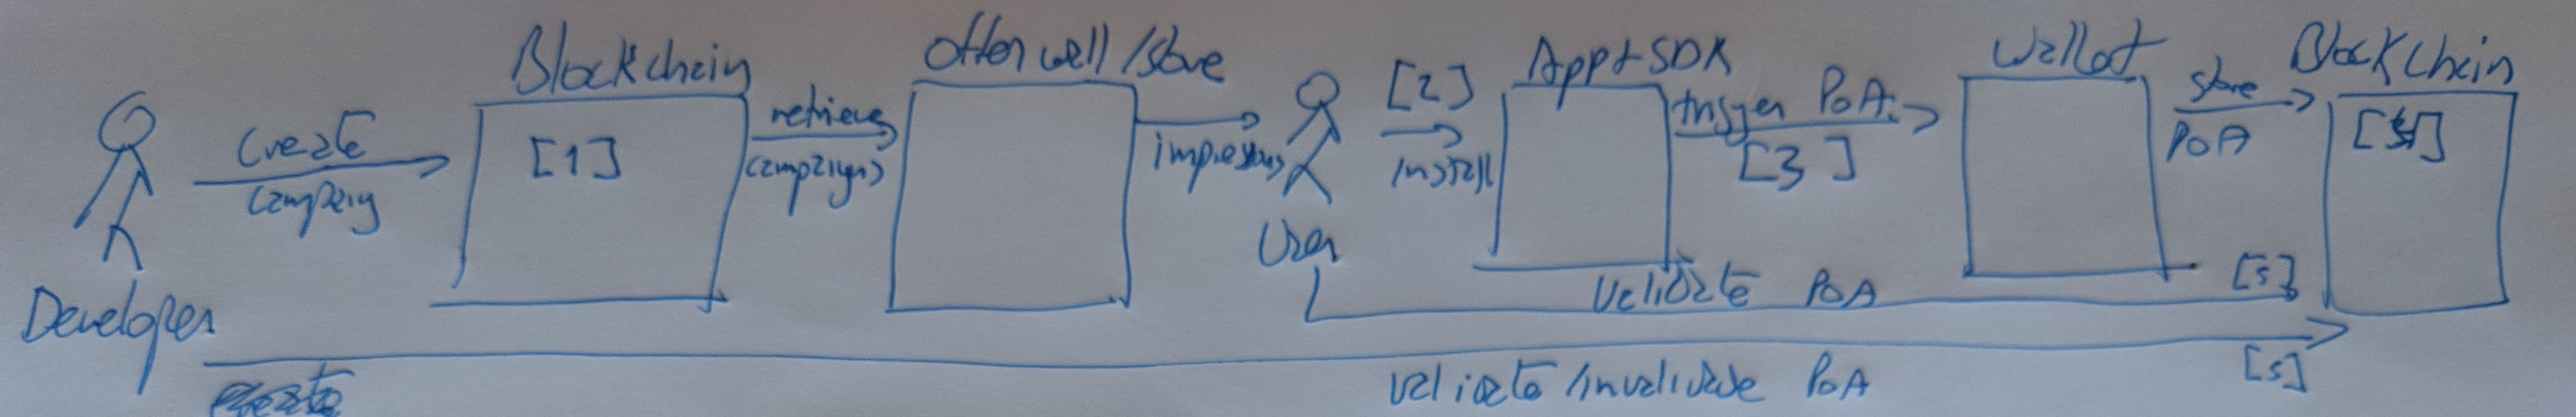
\includegraphics[width=\textwidth]{diagrams/messages_exchanged_diagram.png}
\caption{Messages exchanged in the Advertising use case diagram.}
\label{fig:messages_diagram}
\end{figure}


Figure \ref{fig:ads_sequence_diagram} presents five different objects (data structures and interfaces):

\begin{enumerate}
\item Campaign definition (in the blockchain)
\item Attribution methods interfaces
\item PoA Trigger
\item PoA definition (in the blockchain)
\item PoA validation / invalidation definition (in the blockchain)
\end{enumerate}

\medskip

{\bf [1] Campaign definition (in the blockchain) }

When creating a campaign in step \textsf{(1)} from Figure \ref{fig:ads_sequence_diagram}, the advertiser (developer) specifies the filters that should be used by app stores to select users matching the defined criteria, as well as the validation rules that should be used when a \textsf{PoA} is submitted to verify if it complies with the campaign rules. Therefore, the campaign object has following format:
\begin{tcolorbox}[enhanced jigsaw,sharp corners, drop fuzzy shadow=ShadowColor]
\begin{lstlisting}[xleftmargin=0.05\textwidth]
{
    "campaign_id": "9e850e4ce590f20dc03568f144543741",
    "filters": {
        "country": ["US", "ES", "CA"],
	"package": "cm.aptoide.pt",
	"vercode": [4283,4284]
    },
    "attribution_validation_rules": {
        "vercode": "false",
        "IP_validation_required":"true",
        "country": "true",
        "IP_daily_conversions": 2,
        "wallet_daily_conversions":1
    },
    "price": 1,
    "budget": 10,
    "start_date": "2018-04-23 15:21:19+00:00",
    "end_date": "2018-04-25 15:21:19+00:00",
    "ip_validator": "whoami.developer.com",
    "dev_wallet": "0x59dc842b64c7229af88f8b0b02fdf04ff6f083ad"
}
\end{lstlisting}
\end{tcolorbox}

\medskip

{\bf [2] Attribution methods interfaces}

Regarding the attribution scheme, i.e. the mechanisms by which the SDK knows the wallet addresses of the app store and the OEM that should receive the revenue share attributed to app stores and OEMs for a given attribution, the protocol defines 3 different ways, with different degrees of priority, for the SDK to know the app store and the OEM that should receive the correspondent shares when a valid \textsf{PoA} is produced and sent to the blockchain. For all the 3 possibilities, there is a common component which is a JSON file stored by the wallet consisting of a mapping between app stores and OEM IDs and their respective Ethereum wallet addresses. This file has the following format:
\begin{tcolorbox}[enhanced jigsaw,sharp corners, drop fuzzy shadow=ShadowColor]
\begin{lstlisting}
{
  "stores": {
    "cm.aptoide.pt": "aptoide_address",
    "com.google.vending": "google_address",
    "default_address": "default_address"
  },
  "oems": {
    "xiaomi_oem_id": "xiaomi_address",
    "google_oem_id": "google_address",
    "default_address": "default_address"
  }
}
\end{lstlisting}
\end{tcolorbox} 

Regarding the first possibility, and the one with the highest level of priority, it consists in having the SDK asking the Android Operating System (Android OS) which app installed the one where the SDK is integrated. If the Android OS does not know because the app store, upon installing the app that integrates the SDK, did not inform it, then the second possibility is to have the app store broadcasting its ID and the OEM ID to the SDK. For these two options, when the SDK sends the \textsf{PoA} components to the wallet, it also sends the app store and OEM IDs, which should be mapped to the corresponding Ethereum wallet addresses using the aforementioned JSON file. Lastly, if the app store does not inform the Android OS that it installed the app nor this it send a broadcast upon installation, then the wallet should consider the default addresses for both the app store and the OEM that shall be attributed the share. 


\medskip

{\bf [3] PoA Trigger}


%%  This part is missing. We need to define the intent 

\medskip

{\bf [4] PoA definition}

Regarding the definition of the \textsf{PoA} components sent by the SDK to the wallet in step \textsf{(4)}, they hold data that enable the wallet to aggregate components by package. The format of each component is the following:
\begin{tcolorbox}[enhanced jigsaw,sharp corners, drop fuzzy shadow=ShadowColor]
\begin{lstlisting}[xleftmargin=0.05\textwidth]
{
    "ts": "2018-04-04 12:34:33+00:00",
    "package_name": "com.asfoundation.wallet"
}
\end{lstlisting}
\end{tcolorbox}

As said in step \textsf{(4)}, for each \textsf{PoA} component the wallet should compute a \textit{nonce} in a Bitcoin-style \textsf{PoW} that helps avoiding click spoofing by introducing a computation step that takes a certain amount of time. Given a \textsf{PoA} component as the one above, a \textsf{SHA256} hash $h_C$ is computed and the goal is to find an integer $nonce$ that when concatenated with the hash $h_C$ outputs another \textsf{SHA256} hash $pow$ with a certain number of leading zeros. As an example, assuming the \textsf{PoA} component above and denoting it as $C$:
\begin{tcolorbox}[enhanced jigsaw,sharp corners, drop fuzzy shadow=ShadowColor]
\begin{align*}
h_C &= sha256(C) \\
	    &= 2de1a25b781dda30fae45cb34495501c9fe3fb83f464e46c6d6e19b48f09b440 \\
n_{zeros} &= 5 \\
nonce &= 959928 \\
pow &= sha256(nonce + h_C) \\
		       &= 0000051232895be3f3a541907bcb5e69a87a4b39ebc3c43ee4d1f256b71c8364
\end{align*}
\end{tcolorbox}

After validating 12 \textsf{PoA} components, the wallet computes a full \textsf{PoA}, which is of the form:
\begin{tcolorbox}[enhanced jigsaw,sharp corners, drop fuzzy shadow=ShadowColor]
\begin{lstlisting}[xleftmargin=0.05\textwidth]
{
    "campaign_id": "9e850e4ce590f20dc03568f144543741",
    "poa_id": "x1g45gbhb2d26b0ef3cfbabc16f4553baa267byu",
    "ipvalidation": "signed_ip",
    "package_name": "com.asfoundation.wallet"
    "components": [
                    {"ts": "2018-04-03 16:39:27+00:00",
                     "nonce": 421},
                    {"ts": "2018-04-03 16:39:37+00:00",
                     "nonce": 1345},
                    {"ts": "2018-04-03 16:39:47+00:00",
                     "nonce": 5985},
                    {"ts": "2018-04-03 16:39:57+00:00",
                     "nonce": 3568},
                    {"ts": "2018-04-03 16:40:07+00:00",
                     "nonce": 7030},
                    {"ts": "2018-04-03 16:40:17+00:00",
                     "nonce": 6110},
                    {"ts": "2018-04-03 16:40:27+00:00",
                     "nonce": 2215},
                    {"ts": "2018-04-03 16:40:37+00:00",
                     "nonce": 1793},
                    {"ts": "2018-04-03 16:40:47+00:00",
                     "nonce": 6077},
                    {"ts": "2018-04-03 16:40:57+00:00",
                     "nonce": 1391},
                    {"ts": "2018-04-03 16:41:07+00:00",
                     "nonce": 149},
                    {"ts": "2018-04-03 16:41:17+00:00",
                     "nonce": 3688}
                  ]
}
\end{lstlisting}
\end{tcolorbox}
Note that each component in the full \textsf{PoA} includes the value of its corresponding \textit{nonce} for posterior validation, if needed. The \textit{package\_name} field is passed to the first level fields of the object since it is appears in every component. \\


\medskip

{\bf [5] PoA validation / invalidation definition}

%% This section is missing. Is very similar but it has to state what are the format for the invalidation messages in the blockchain

%% The invalidation has to be very clear about while rule was not match and identify why the attribution failed



\subsection{In-App Billing}
%missing intro?

\subsubsection{Use Case Flows}

Figure \ref{fig:iab_sequence_diagram} shows how the different parties taking part in the IAB use case interact.

\begin{figure}[H]
\centering
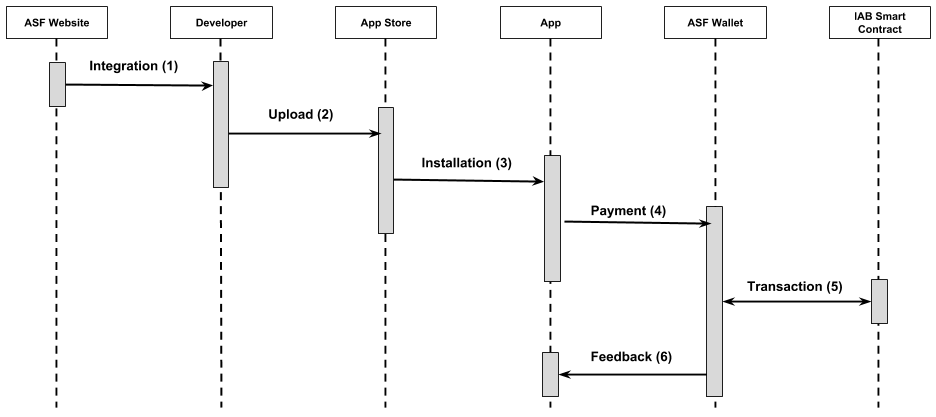
\includegraphics[width=\textwidth]{diagrams/iab_sequence_diagram.png}
\caption{Sequence diagram of the IAB use case.}
\label{fig:iab_sequence_diagram}
\end{figure}

There are several interactions taking place in the IAB use case, although only interactions \textsf{4}, \textsf{5} and \textsf{6} are expected to occur several times during the lifecycle of an app. \\

\noindent \textbf{Integration (1)}. This refers to the integration of the SDK in the app by the developer. During the SDK integration, the developer specifies the SKUs and related information, as well as the ETH account that shall receive the payments when users by in-app items. Therefore, the integration is very simple and does not require much implementation from the developer. \\

\noindent \textbf{Upload (2) \& Installation (3)}. When the developer finishes the integration of the SDK, the resulting APK needs to be uploaded to the app store, since the distribution of apps is done by the several app stores that integrate the AppCoins protocol. Users then install the apps from the app stores. At the moment of the installation, the app store communicates that the app was installed by it. This communication is key to make the app store eligible to take part in the IAB revenue share model and is done either by having the app store broadcasting this data to the SDK or by having it inform the OS of the device that it installed the app. From the app store ID now stored in the SDK, the mapping between this app store ID and the correspondent ETH account can be made by the wallet, since it stores a file with a mapping between the several AppCoins compliant app stores IDs and their ETH accounts. The file is a JSON file of the form:
\begin{tcolorbox}[enhanced jigsaw,sharp corners, drop fuzzy shadow=ShadowColor]
\begin{lstlisting}
{
  "stores": {
    "cm.aptoide.pt": "aptoide_address",
    "com.google.vending": "google_address"
  },
  "oems": {
    "xiaomi_oem_id": "xiaomi_address",
    "google_oem_id": "google_address"
  },
  "default_address": "default_address"
}
\end{lstlisting}
\end{tcolorbox} 

\vspace{0.2cm} \noindent \textbf{Payment (4)}. Whenever a user wants to buy an in-app item, the SDK triggers the payment flow. This payment flow is composed by a verification step to ensure an AppCoins compliant wallet is installed in the user's device and by a payment intent that should be caught by an AppCoins compliant wallet. If the no such wallet is installed, then user is directed to a place where it is possible to download one. An AppCoins compliant wallet is characterised by the implementation of the ERC-681\footnote{https://github.com/ethereum/EIPs/blob/master/EIPS/eip-681.md} with the format:
\begin{lstlisting}
ethereum:target_address?function=iab_pay(args)
args := (amount, prod_id, dev_addr, store_addr, oem_addr)
\end{lstlisting}

If there is a wallet installed that is listening to intents with the above format, the payment request is sent to it. The wallet is then responsible to process the intent and trigger the actual Ethereum transaction following the IAB revenue share model. \\

\noindent \textbf{Transaction (5)}. When the wallet receives the payment intent, the intent contains the amount of APPC the in-app item costs and its ID, and the ETH addresses of the developer of the app, the app store that distributed the app and the OEM that pre-loaded the app store. The wallet calls the smart contract that computes the revenue share for each of the players involved, triggers an event to store in the blockchain that the payment of the in-app item and then triggers the transfers for the developer, the app store and the OEM. \\

\noindent \textbf{Feedback (6)}. When the wallet triggers the payments, it then checks if they were accepted by the Ethereum network in order to give feedback to the app that the transactions are done. It then sends back the status of the transactions and their ID to the SDK in the app for further verification and acceptance.

\subsubsection{Use Case Format Definition}
\label{sssec:iab_fd}

\subsubsection{Data Structures}

\noindent \textbf{IAB Ledger}. The \textit{IAB ledger} is the record of items bought by users. It records transactions in a way that anyone can verify an anonymous user bought a quantity $Q$ of an item $I$ for a price $P$ from an app that integrated the IAB solution from app store $AS$.
\begin{table}[H]
\footnotesize
\centering
\begin{tabular}{|p{1.0\textwidth}|}
\hline
\multicolumn{1}{|c|}{Data Structures} \\
\hline \vspace{0.05cm}
\textbf{IAB Ledger} \\
IAB ledger $L_{IAB} : (TX_1..TX_n)$
\begin{itemize}
	\item Transaction $TX_i$, a transaction stating that an anonymous user $u$ bought a quantity $Q$ an item $I$ with price $P$ from an app $A$ that integrated the IAB solution from app store $AS$
\end{itemize} \\
\hline
\end{tabular}
\caption{Data Structures for IAB Use Case}
\label{table: data_structures_iab}
\end{table}


\subsubsection{Algorithms' Pseudo-code}

\noindent \textsf{Create transaction}. When a user $u$ wants to buy a certain amount $Q$ of items $I$, a transaction is created stating that the user $u$ bought a quantity $Q$ of an item $I$ for a price $P$ in a app $A$ that integrated the IAB solution from app store $AS$. \\

$\left[\begin{tabular}{p{.7\textwidth}}
\textsf{IAB.CreateTransaction}
\begin{itemize}
	\item INPUTS:
	\begin{itemize}
		\item User $u$
		\item Item $I$
		\item App $A$
		\item Developer $D$
		\item App store $AS$
		\item OEM $O$
	\end{itemize}
	\item OUTPUTS: Result $R$ (0 or 1)
\end{itemize}
\vspace{-0.8cm}
\end{tabular}\right.$ \\

\begin{table}[H]
\scriptsize
\centering
\begin{tabular}{|p{0.7\textwidth}|}
\hline
\multicolumn{1}{|c|}{IAB Use Case} \\
\hline \vspace{0.1cm}
\textsf{IAB.CreateTransaction}
\vspace{-0.3cm}
\begin{itemize}
	\item INPUTS:
	\vspace{-0.4cm}
	\begin{itemize}
		\item User $u$
		\item Item $I$
		\item App $A$
		\item Developer $D$
		\item App store $AS$
		\item OEM $O$
	\end{itemize}
	\item OUTPUTS: Result $R$ (0 or 1)
\end{itemize}
\begin{enumerate}
	\item Compute $TX$ := \textsf{Transaction}($u$,$I$,$D$,$AS$,$O$)
	\item Compute $R$ := \textsf{WriteIABLedger}($TX$)
	\item if $R = 1$:
	\begin{enumerate}
		\item App $A$ issues items to user
		\item Compute $(T_D, T_{OEM}, T_{AS})$ := \textsf{DivideTokens}($F$)
		\item Send $T_D$ to developer's wallet $W_D$
		\item Send $T_{OEM}$ to OEM's wallet $W_{OEM}$
		\item Send $T_{AS}$ to user's wallet $W_{AS}$
	\end{enumerate}
\end{enumerate} \\
\hline
\end{tabular}
\caption{IAB Use Case. In \textsf{CreateTransaction}, the issuing of items in certain app $A$ is purely done in the app based on the result of the method, since the items are not in the blockchain and there is no real blockchain transaction happening.}
\label{table: iab_protocol}
\end{table}


\subsubsection{Wallet Transactions}

In In-App Billing the transactions between wallets occur off-chain. The main transactions are between the user that is buying the digital item and 3 recipients: the developer, the OEM and the app store. Figure \ref{fig:wallet_iab_flow} presents the different flows of IAB transactions.

\begin{figure}[!ht]
\centering
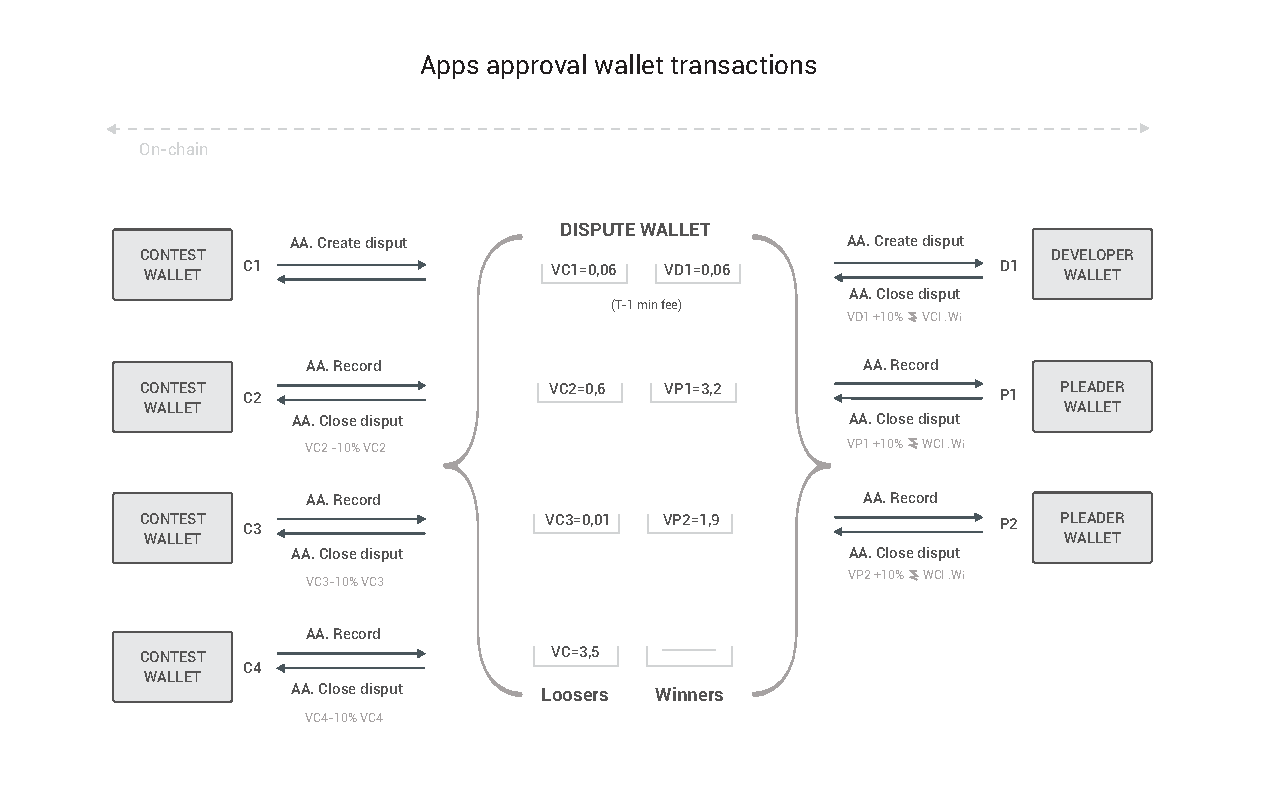
\includegraphics[width=0.85\textwidth]{diagrams/wallet_transfers_iab.eps}
\caption{Wallet transfers in IAB flow.}
\label{fig:wallet_iab_flow}
\end{figure}


\subsection{Developer Rank}
\label{subsec:protocol_devrank}

There is the need to create trust between the different players in the app economy, namely between users, the developers and their apps. \\

In the AppCoins protocol, trust is characterised by a developer's rank, which is then propagated to all his apps. This rank can have the values of $\{"Unknown", "Trusted", "Critical"\}$. A user has the rank \textit{"Unknown"} only when joining the network for the first time, i.e. once the rank is changed from \textit{"Unknown"}, it can never have this value again. Changes in rank happen either through disputes, where the rank of the developer can change to \textit{"Critical"} in case of loss or remain the same in case of win, or by promotions, where the rank of the developer can change to \textit{"Trusted"}.

Promotions depend on the number of transactions in each of the developer's apps compared to the number of transactions in other popular apps. Promotions are automatic and depend on the following condition:

\begin{equation}
\sum\limits_{t=0}^{T} \sum\limits_{i=1}^{N} TX_{A_{ij},t} \geq TX_{A^{T}_{M}}
%T variable in the date and part of TX is confusing looks like T multiplied by X
\label{eq: promo_cond}
\end{equation}

Where $A_i = \{A_{i1}..A_{iN}\}$ is the set of N apps of developer $D_i$, meaning that $A_{ij}$ is the app $j$ in the set $A_i$, $t$ is the day with $t=0$ being the moment the developer joined the network, $T$ is the current day, $A^{T}_{M}$ is the app with the highest number of transactions on day $T$. Given these variables definitions, one can see that the left side in Equation \ref{eq: promo_cond} represents the amount of transactions in all the apps of developer $D_i$ since he joined the network and the right side represents the number of transactions of the app with the highest number of transactions on day $T$.

Contrary to the promotions, disputes are not done automatically and require explicit actions from users. Any user can open a dispute with a developer stating that the developer is dishonest. After the dispute is opened, any other user can join either side, depending on if they want to support the accusation of dishonesty or if they want to defend the developer.

Additionally, each rank value has a level associated with it. For \textit{"Unknown"} and \textit{"Critical"} rank values, the level is always set to 1. When the rank is \textit{"Trusted"}, we do not set a maximum level and it is expressed by:
\begin{equation}
S_l = \log_2 \frac{\sum\limits_{t=0}^{T} \sum\limits_{i=1}^{N} TX_{A_{ij},t}}{TX_{A^{T}_{M}}}
\label{eq: rank_level}
\end{equation}

Because of the use of the logarithm function in Equation \ref{eq: rank_level}, it becomes harder to gain higher rank levels as the rank level increases.

\subsubsection{Developer Reputation}

%A known developer is more trustable than a developer recently arrived to the apps' distribution business.
It is assumed that a known developer is more trustworthy than a developer who recently joined the apps distribution business.

\subsubsection{Data Structures}

\noindent \textsf{Dispute Intent}. A \textit{dispute intent} happens when a user claims that a developer is dishonest and no dispute against that developer is open. The developer or any other user then has 7 days to answer the dispute. If someone answers the dispute, be it the developer or any other user, the dispute is opened and the minimum fees needed to open it are captivated. If no user answers the dispute, the \textit{dispute intent} closes and the developer status changes to \textit{critical}. \\
%in the last sentence "If no user answers the dispute". Shouldn't it be "If no user or developer answers the dispute" else a user can allways blacklist any developer provided that other users don't reply

\noindent \textsf{Dispute}. A \textit{dispute} is a conflict between two parties, where one party - the \textit{contestants} - claim that a developer is dishonest, i.e. the developer uploads apps with malware, too many ads, or non-working apps and the other party - the \textit{pleaders} - claim the developer is honest. The pleaders include the developer being accused of dishonesty by the contestants. Both parties place tokens in the dispute and the party holding the most amount of tokens by the end of the dispute wins. Therefore, the \textit{dispute} includes the developer it regards to, the participants in both parties and their respective stake in the dispute. \\
%how many tokens each user, developer puts?

\noindent \textsf{DisputeLedger}. The \textit{dispute ledger} is the record of users joining disputes. It stores that a user joined a dispute on behalf of one of the sides with a certain stake (amount of tokens). The entries in the \textit{dispute ledger} are used to settle disputes when they end. \\

\noindent \textsf{RankLedger}. The \textit{rank ledger} is the record of rank changes of developers. Whenever there is a change in a developer's rank, be it an increase in the \textit{"Trusted"} rank levels or a change to \textit{"Critical"}, it is recorded in the \textit{rank ledger}.

\begin{table}[H]
\footnotesize
\centering
\begin{tabular}{|p{1.0\textwidth}|}
\hline
\multicolumn{1}{|c|}{Data Structures} \\
\hline \vspace{0.05cm}
\textbf{DisputeIntent} \\
dispute intent $K^{0}_{x} := \langle D_i, C_j, T_{min}, S\rangle$
\begin{itemize}
	\item Developer $D_i$, the developer being accused of being dishonest
	\item Contestant $C_j$, user claiming developer $D_i$ is dishonest
	%C has been defined as campaign
	\item Minimum fee $T_{min}$, the minimum fee needed to open the dispute that may result from this dispute intent
	\item status $S$, the current status of the dispute intent, which can take the values of \textit{"Open"} or \textit{"Closed"}
\end{itemize} \\
\textbf{Dispute} \\
dispute $K_x := \langle D_i, S, T_{min}\rangle$
\begin{itemize}
	\item Developer $D_i$, the developer being accused of being dishonest
	\item status $S$, the current status of the dispute, which can take the values of \textit{"Open"} or \textit{"Closed"}
	\item Minimum fee $T_{min}$, the minimum fee needed to open the dispute
	%who defines the value of $T_{min}$, dows it change between disputes?
\end{itemize} \\
\textbf{Dispute Ledger} \\
dispute ledger $L_{K} : (E_1..E_n)$
\begin{itemize}
	\item entry $E_i$, an entry containing information about a user joining a dispute in the form $E_i := \langle U_i, P, T, K_x\rangle$, where $U_i$ is the user, $P$ is the position the user is taking (can be either \textit{"Contestants"} or \textit{"Pleaders"}), $T$ is the stake (amount of tokens) the user $U_i$ is willing to use to defend position $P$ and $K_x$ is the dispute user $U_i$ is joining
\end{itemize} \\
\textbf{Rank Ledger} \\
rank ledger $L_{R} : (E_1..E_n)$
\begin{itemize}
	\item entry $E_i$, an entry containing information about a change in a developer's rank in the form $E_i := \langle D_i, S_b, S_a, S_l\rangle$, where $D_i$ is the developer, $S_b$ is the developer's rank before the change, $S_a$ is the rank after the change and $S_l$ is the level of the rank. $S_b$ can take the values of $\{"Unknown", "Trusted"\}$ and $S_a$ can take the values of $\{"Trusted", "Critical"\}$. For further details regarding the possible states of $S_b$ and $S_a$ and the possible values of $S_l$, please refer to Figure \textbf{[INCLUDE REF TO FIG]}.
\end{itemize} \\
\hline
\end{tabular}
\caption{Data Structures for Developers Rank Use Case}
\label{table: data_structures_da}
\end{table}


\subsubsection{Algorithms' Pseudo-code}

%user was previously $U$
%what are i,j,z,x ans 0
\noindent \textbf{Create dispute intent}. When a user $C_i$ claims a developer $D_j$ is dishonest, an intent of dispute is created, which may result in a dispute being opened, depending on whether someone answers the \textit{dispute intent} within 7 days or not. The user answering the dispute may not be the developer. \\

$\left[\begin{tabular}{p{.7\textwidth}}
\textsf{DR.CreateDisputeIntent}
\begin{itemize}
	\item INPUTS:
	\begin{itemize}
		\item User $C_z$
		\item Developer $D_j$
	\end{itemize}
	\item OUTPUTS: Dispute intent $K^{0}_{x}$
\end{itemize}
\vspace{-0.8cm}
\end{tabular}\right.$ \\

\noindent \textbf{Create dispute}. When a dispute intent is answered, a disputed is created. Within the following 30 days, any user may join the contestants side, which is composed by users claiming the developer $D_j$ is dishonest, or the pleaders side, which contains users stating that the developer $D_j$ is honest. The dispute intent that originated the new dispute is closed.\\

$\left[\begin{tabular}{p{.7\textwidth}}
\textsf{DR.CreateDispute}
\begin{itemize}
	\item INPUTS:
	\begin{itemize}
		\item Developer $D_j$
		\item Minimum fee $T_{min}$
		\item Dispute intent $K^{0}_{x}$
	\end{itemize}
	\item OUTPUTS: Dispute $K_x$
\end{itemize}
\vspace{-0.8cm}
\end{tabular}\right.$ \\

\noindent \textbf{Close dispute}. When the dispute is over (after 30 days), the winning side has its stakes refunded, while also receiving 10\% of each pledge from the losing side, with each winning member getting a winning stake proportional to their stake in the overall winning side pledge. Each member from the losing side gets a refund from the respective pledge subtracted by 10\%. Please refer to Table \ref{table: dr_protocol} for more details. \\

$\left[\begin{tabular}{p{.7\textwidth}}
\textsf{DR.CloseDispute}
\begin{itemize}
	\item INPUTS:
	\begin{itemize}
		\item Dispute $K_x$
	\end{itemize}
	\item OUTPUTS: None
\end{itemize}
\vspace{-0.8cm}
\end{tabular}\right.$ \\

\noindent \textbf{Compute rank}. The rank of the developer is periodically checked to assess changes in its value. For example, the rank can change from \textit{"Unknown"} to \textit{"Trusted"} or the \textit{"Trusted"} level can increase. \\

$\left[\begin{tabular}{p{.7\textwidth}}
\textsf{DR.ComputeRank}
\begin{itemize}
	\item INPUTS:
	\begin{itemize}
		\item Developer $D_i$
		\item Set of transactions in developer's apps $TX_i$
		\item Set of developer's apps $A_i$
		\item App with the highest amount of transactions $A_M$
	\end{itemize}
	\item OUTPUTS: None
\end{itemize}
\vspace{-0.8cm}
\end{tabular}\right.$ \\

\noindent \textbf{Record dispute}. When a user joins a side on a dispute, the event is recorded in the dispute ledger and can later be used to settle the dispute. \\

$\left[\begin{tabular}{p{.7\textwidth}}
\textsf{DR.RecordDispute}
\begin{itemize}
	\item INPUTS:
	\begin{itemize}
		\item User $U_i$
		\item Position $P$
		\item Stake $T$
		\item Dispute $K_x$
	\end{itemize}
	\item OUTPUTS: None
\end{itemize}
\vspace{-0.8cm}
\end{tabular}\right.$ \\

\noindent \textbf{Record rank change}. When there is a developer's rank change, it is recorded in the rank ledger. \\

$\left[\begin{tabular}{p{.7\textwidth}}
\textsf{DR.RecordRank}
\begin{itemize}
	\item INPUTS:
	\begin{itemize}
		\item Developer $D_i$
		\item New rank $S_a$
		\item New rank level $S_l$
	\end{itemize}
	\item OUTPUTS: None
\end{itemize}
\vspace{-0.8cm}
\end{tabular}\right.$ \\

\begin{table}[H]
\scriptsize
\centering
\begin{tabular}{|p{.5\textwidth}p{.5\textwidth}|}
\hline
\multicolumn{2}{|c|}{Developers' Rank Use Case} \\
\hline \vspace{0.1cm}
\textsf{DR.CreateDisputeIntent}
\vspace{-0.3cm}
\begin{itemize}
	\item INPUTS:
	\vspace{-0.3cm}
	\begin{itemize}
		\item User $C_z$
		\item Developer $D_j$
	\end{itemize}
	\item OUTPUTS: Dispute intent $K^{0}_{x}$
\end{itemize}
\begin{enumerate}
	\item Compute $K^{0}_{x}$ := \textsf{DisputeIntent}($D_j$, $C_z$)
	\item Set $K^{0}_{x}$.Status := \textit{"Open"}
\end{enumerate} & \vspace{0.1cm}
\textsf{DR.CreateDispute}
\vspace{-0.3cm}
\begin{itemize}
	\item INPUTS:
	\vspace{-0.3cm}
	\begin{itemize}
		\item Developer $D_j$
		\item Minimum fee $T_{min}$
		\item Dispute intent $K^{0}_{x}$
	\end{itemize}
	\item OUTPUTS: Dispute $K_x$
\end{itemize}
\begin{enumerate}
	\item Set $K^{0}_{x}$.Status := \textit{"Closed"}
	\item Compute $K_x$ := \textsf{Dispute}($D_j$, $T_{min}$)
	\item Set $K_x$.Status := \textit{"Open"}
\end{enumerate} \\ \vspace{0.1cm}
\textsf{DR.CloseDispute} 
\vspace{-0.3cm}
\begin{itemize}
	\item INPUTS:
	\vspace{-0.3cm}
	\begin{itemize}
		\item Dispute $K_x$
	\end{itemize}
	\item OUTPUTS: None
\end{itemize}
\begin{enumerate}
	\item Compute $WinSide$ := \textsf{WinningSide}($K_x$)
	\item Compute \textsf{DistributePledges}($K_x$)
	\item Set $K_x$.Status := \textit{"Closed"}
	\item If $WinSide$ = \textit{"Contestants"}:
	\begin{enumerate}
		\item Compute \textsf{DR.RecordRank}($K_x$.D, \textit{"Critical"}, 1)
	\end{enumerate}
\end{enumerate} & \vspace{0.1cm}
\textsf{DR.ComputeRank} 
\vspace{-0.3cm}
\begin{itemize}
	\item INPUTS:
	\vspace{-0.3cm}
	\begin{itemize}
		\item Developer $D_i$
		\item Set of transactions in developer's apps $TX_i$
		\item Set of developer's apps $A_i$
		\item App with the highest amount of transactions $A_M$
	\end{itemize}
	\item OUTPUTS: None
\end{itemize}
\begin{enumerate}
	\item Compute $S_l$ := \textsf{RankLevel}($TX_i$, $A_M$)
	\item If $S_l \geq 1$ and $D_i$.Rank = \textit{"Unknown"}:
	\begin{enumerate}
		\item Compute \textsf{DR.RecordRank}($D_i$, \textit{"Trusted"}, $S_l$)
		\item Return
	\end{enumerate}
	\item If $S_l > D_i$.RankLevel and $D_i$.Rank = \textit{"Trusted"}:
	\begin{enumerate}
		\item Compute \textsf{DR.RecordRank}($D_i$, \textit{"Trusted"}, $S_l$)
		\item Return
	\end{enumerate}
\end{enumerate} \\ \vspace{0.1cm}
\textsf{DR.RecordDispute}
\vspace{-0.3cm}
\begin{itemize}
	\item INPUTS:
	\vspace{-0.3cm}
	\begin{itemize}
		\item User $U_i$
		\item Position $P$
		\item Stake $T$
		\item Dispute $K_x$
	\end{itemize}
	\item OUTPUTS: None
\end{itemize}
\begin{enumerate}
	\item Send $T$ from user $U_i$ wallet $W_{U_i}$ to dispute's wallet $W_{K_x}$
	\item Set $E := \langle U_i, P, T, K_x\rangle$
	\item Compute \textsf{WriteDisputeLedger}($E$)
\end{enumerate} & \vspace{0.1cm}
\textsf{DR.RecordRank}
\vspace{-0.3cm}
\begin{itemize}
	\item INPUTS:
	\vspace{-0.3cm}
	\begin{itemize}
		\item Developer $D_i$
		\item New rank $S_a$
		\item New rank level $S_l$
	\end{itemize}
	\item OUTPUTS: None
\end{itemize}
\begin{enumerate}
	\item Set $S_b$ := $D_i$.Rank
	\item Set $E := \langle D_i, S_b, S_a, S_l\rangle$
	\item Compute \textsf{WriteRankLedger}($E$)
\end{enumerate} \\
\hline
\end{tabular}
\caption{Developers Rank Use Case}
\label{table: dr_protocol}
\end{table}


\subsubsection{Wallet Transactions}

The reputation of a developer is built based on blockchain transactions that can be associated to him. However, when there is a dispute, as presented in the previous section, the dispute mechanism is solved by receiving positive / negative endorsements of the community members to the developer. The final decision is based on the total sum of tokens that each side has. Figure \ref{fig:wallet_developers_approval} shows how users create disputes and join sides by placing tokens on the dispute.
%how many tokens each user and developer puts? Is it a fixed value? If variable, can rich malware developers or users takeover the system?

\begin{figure}[!ht]
\centering
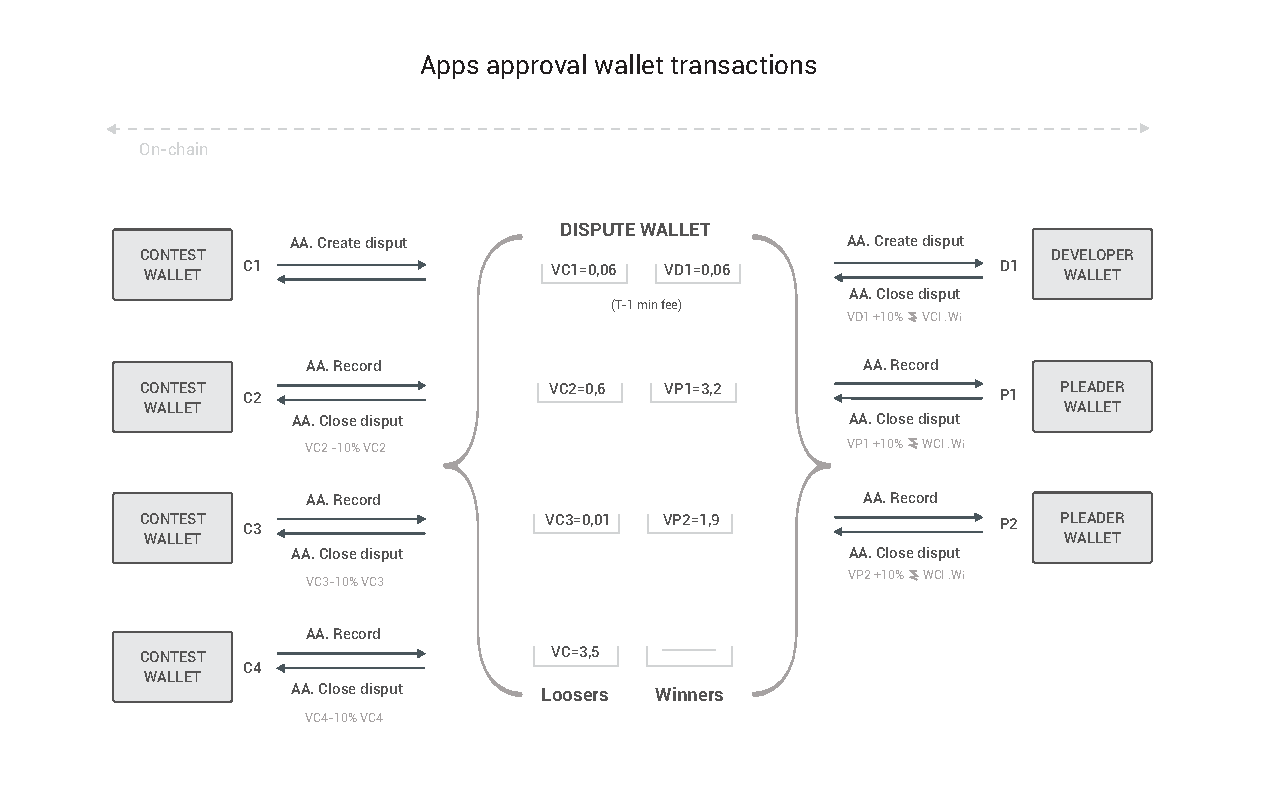
\includegraphics[width=\textwidth]{diagrams/wallet_transfers_approval.eps}
\caption{Wallet transfers in the Developers Approval process.}
\label{fig:wallet_developers_approval}
\end{figure}


% descrever esta área após recebimeto do diagrama








